\documentclass[tikz,border=5pt]{standalone}
\usepackage{amsmath, amssymb}
\usepackage{tikz}
\usetikzlibrary{shapes.geometric, positioning}

\begin{document}

    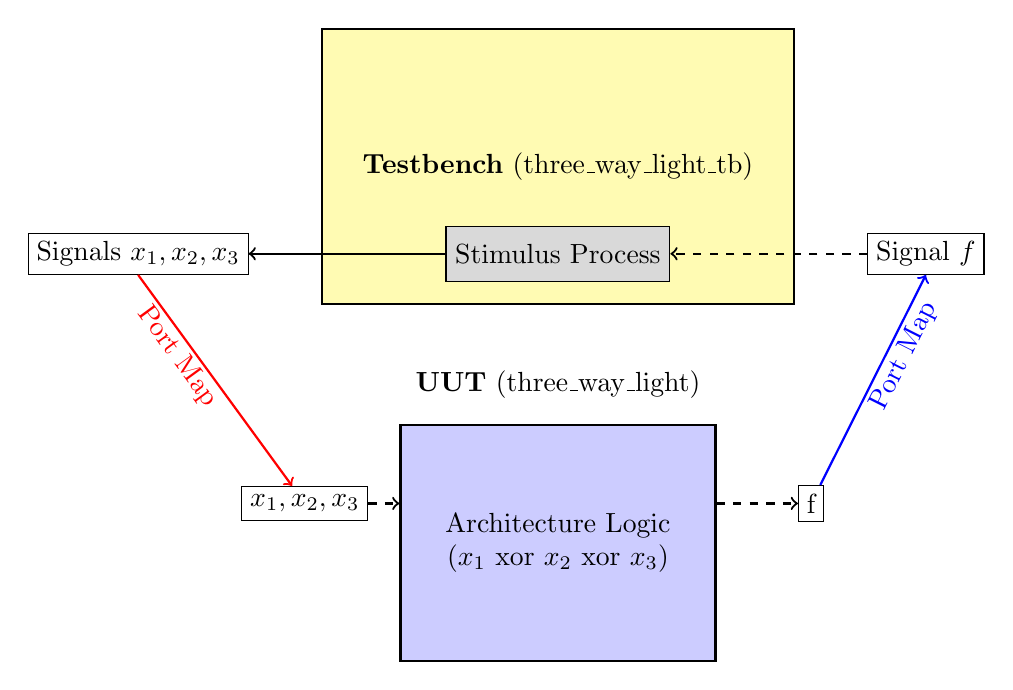
\begin{tikzpicture}[
        TB/.style={rectangle, draw=black, fill=yellow!30, minimum width=6cm, minimum height=3.5cm, align=center, thick},
        UUT/.style={rectangle, draw=black, fill=blue!20, minimum width=4cm, minimum height=3cm, align=center, thick},
        Process/.style={rectangle, draw=black, fill=gray!30, align=center, minimum height=0.7cm},
        Signal/.style={coordinate},
        Port/.style={rectangle, draw=black, fill=white, inner sep=3pt}
    ]

    % Draw the Testbench (three_way_light_tb)
    \node (TB) [TB] {\textbf{Testbench} ($\text{three\_way\_light\_tb}$)};
    
    % Draw the Stimulus Process within the Testbench
    \node (Stim) [Process, above=0.3cm of TB.south, anchor=south, xshift=0cm] {Stimulus Process};
    
    % Draw the UUT (three_way_light)
    \node (UUT) [UUT, below=1.5cm of TB] {};
    \node[align=center, yshift=0.5cm] at (UUT.north) {\textbf{UUT} ($\text{three\_way\_light}$)};
    
    % Define the I/O Ports of the UUT
    \node (UUT_IN) [Port, left=1.2cm of UUT.west, anchor=center, yshift=0.5cm] {$x_1, x_2, x_3$};
    \node (UUT_OUT) [Port, right=1.2cm of UUT.east, anchor=center, yshift=0.5cm] {f};

    % Define the Signals in the Testbench
    \node (SIG_IN) [Signal, above right=0.3cm and 0.5cm of Stim.east] {};
    \node (SIG_OUT) [Signal, right=0.3cm of UUT_OUT.east, yshift=0.5cm] {};
    
    \node (SIG_IN_L) [Port, left=2.5cm of Stim.west, yshift=0cm] {Signals $x_1, x_2, x_3$};
    \node (SIG_OUT_L) [Port, right=2.5cm of Stim.east, yshift=0cm] {Signal $f$};
    
    % Draw Internal Testbench Signals/Connections
    \draw[->, thick] (Stim) -- (SIG_IN_L);
    \draw[->, thick, dashed] (SIG_OUT_L) -- (Stim); % Assuming a monitor process in Stim
    
    % Draw connections from Testbench Signals to UUT Ports (Port Map)
    \draw[->, thick, red] (SIG_IN_L.south) -- node[above, sloped, near start, xshift=0.3cm, yshift=-0.5cm] {Port Map} (UUT_IN);
    \draw[->, thick, blue] (UUT_OUT) -- node[above, sloped, near end, xshift=-0.3cm, yshift=-0.5cm] {Port Map} (SIG_OUT_L.south);
    
    % Draw internal UUT connection
    \draw[->, thick, dashed] (UUT_IN) -- (UUT.west |- UUT_IN.center);
    \draw[->, thick, dashed] (UUT.east |- UUT_OUT.center) -- (UUT_OUT);

    % Add labels for the Testbench area
    \node[anchor=south west] at (TB.south west) {};
    
    % Add the logic block inside UUT
    \node[align=center, text width=3cm] at (UUT.center) {Architecture Logic \\ ($x_1$ xor $x_2$ xor $x_3$)};

    \end{tikzpicture}

\end{document}